\documentclass{article}
\usepackage[utf8]{inputenc}
\usepackage[french]{babel}
\usepackage{graphicx}
\usepackage{listings}
\usepackage{color}
\usepackage{hyperref}
\usepackage{geometry}
\usepackage{titling}
\usepackage{fancyhdr}
\geometry{a4paper, margin=2.5cm}

% Configuration des listings pour le code
\definecolor{codegreen}{rgb}{0,0.6,0}
\definecolor{codegray}{rgb}{0.5,0.5,0.5}
\definecolor{codepurple}{rgb}{0.58,0,0.82}
\definecolor{backcolour}{rgb}{0.95,0.95,0.92}

\lstdefinestyle{mystyle}{
    backgroundcolor=\color{backcolour},   
    commentstyle=\color{codegreen},
    keywordstyle=\color{magenta},
    numberstyle=\tiny\color{codegray},
    stringstyle=\color{codepurple},
    basicstyle=\ttfamily\footnotesize,
    breakatwhitespace=false,         
    breaklines=true,                 
    captionpos=b,                    
    keepspaces=true,                 
    numbers=left,                    
    numbersep=5pt,                  
    showspaces=false,                
    showstringspaces=false,
    showtabs=false,                  
    tabsize=2
}

\lstset{style=mystyle}

% Personnalisation de la page de titre
\title{\Huge{\textbf{TP 6 : Intégration Jenkins-Ansible}}}
\author{\Large{Ahmed Abd Dayem Ahmed Bouha} \\ \\ \large{Matricule : \textbf{23243}} \\ \vspace{2cm} \large{Matière : \textbf{IRT43: DevOps}}}
\date{\today}

\begin{document}

% Page de titre personnalisée
\begin{titlepage}
    \centering
    \vspace*{2cm}
    {\Huge\bfseries TP 6 : Intégration Jenkins-Ansible\par}
    \vspace{2cm}
    {\LARGE\bfseries Ahmed Abd Dayem Ahmed Bouha\par}
    \vspace{0.5cm}
    {\large Matricule : \textbf{23243}\par}
    \vspace{1.5cm}
    {\large Matière : \textbf{IRT43: DevOps}\par}
    \vspace{1.5cm}
    {\large\today\par}
    \vspace{1.5cm}
    {\LARGE\bfseries Professeur : Dr. Fatimetou Abdou\par}
    \vspace{1cm}
\end{titlepage}

\tableofcontents
\thispagestyle{empty}
\newpage

\setcounter{page}{1}
\section{Introduction}
Ce rapport présente la réalisation du TP 6 portant sur l'intégration de Jenkins avec Ansible pour automatiser le déploiement d'applications depuis GitHub. Ce projet démontre la mise en place d'un pipeline CI/CD complet qui permet d'extraire du code source depuis un dépôt GitHub et de le déployer automatiquement sur des serveurs cibles à l'aide d'Ansible.

\subsection{Objectifs du TP}
Les principaux objectifs de ce travail pratique sont les suivants :
\begin{itemize}
    \item Configurer Jenkins avec les plugins nécessaires
    \item Créer un pipeline Jenkins qui s'intègre avec GitHub
    \item Automatiser le déploiement d'une application web avec Ansible
    \item Implémenter une solution CI/CD complète
\end{itemize}

\section{Environnement de travail}
\subsection{Configuration système}
\begin{itemize}
    \item Système d'exploitation : Linux 6.12.10-76061203-generic
    \item Shell : /usr/bin/bash
\end{itemize}

\subsection{Outils utilisés}
\begin{itemize}
    \item Jenkins : pour l'orchestration du pipeline CI/CD
    \item Ansible : pour l'automatisation du déploiement
    \item GitHub : pour héberger le code source
    \item Apache : comme serveur web pour l'application déployée
\end{itemize}

\section{Installation et configuration de Jenkins}
\subsection{Installation de Jenkins}
% Étape 1: Installer Jenkins

% Ici, vous ajouterez la capture d'écran de l'installation de Jenkins
\begin{figure}[h]
    \centering
    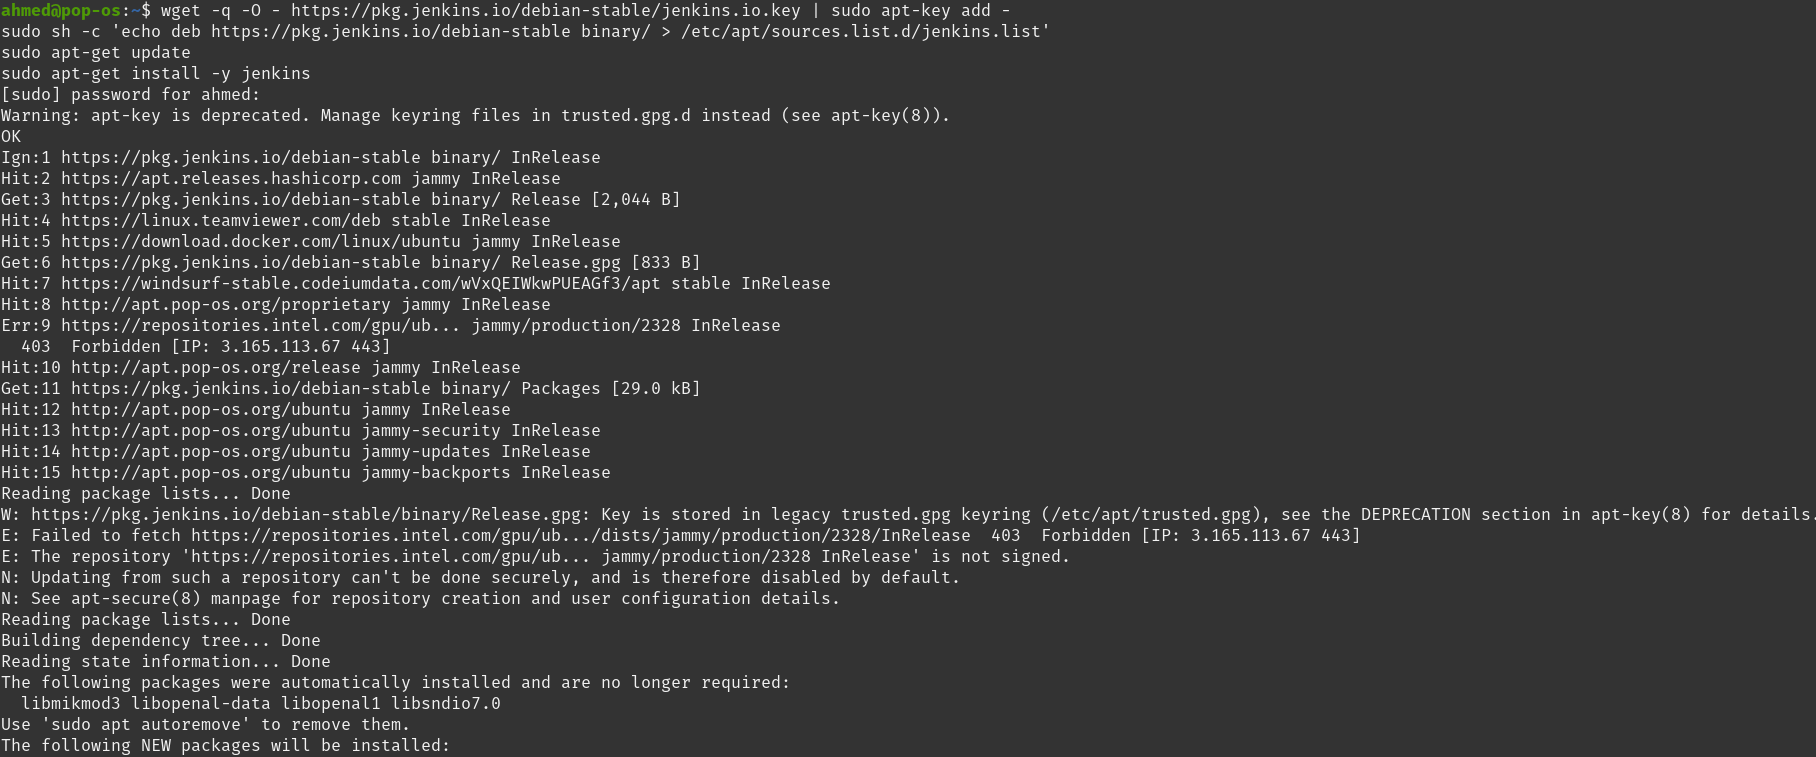
\includegraphics[width=0.8\textwidth]{images/jenkins_installation.png}
    \caption{Installation de Jenkins}
    \label{fig:jenkins_installation}
\end{figure}

J'ai commencé par installer Jenkins en suivant les commandes recommandées :

\begin{lstlisting}[language=bash]
wget -q -O - https://pkg.jenkins.io/debian-stable/jenkins.io.key | sudo apt-key add -
sudo sh -c 'echo deb https://pkg.jenkins.io/debian-stable binary/ > /etc/apt/sources.list.d/jenkins.list'
sudo apt-get update
sudo apt-get install -y jenkins
\end{lstlisting}

Après l'installation, j'ai vérifié que le service Jenkins était bien en cours d'exécution :

\begin{lstlisting}[language=bash]
sudo systemctl status jenkins
\end{lstlisting}

\subsection{Configuration initiale}
Pour la configuration initiale de Jenkins, j'ai récupéré le mot de passe administrateur initial :

\begin{lstlisting}[language=bash]
sudo cat /var/lib/jenkins/secrets/initialAdminPassword
\end{lstlisting}

% Ici, vous ajouterez la capture d'écran de la page de déverrouillage Jenkins
\begin{figure}[h]
    \centering
    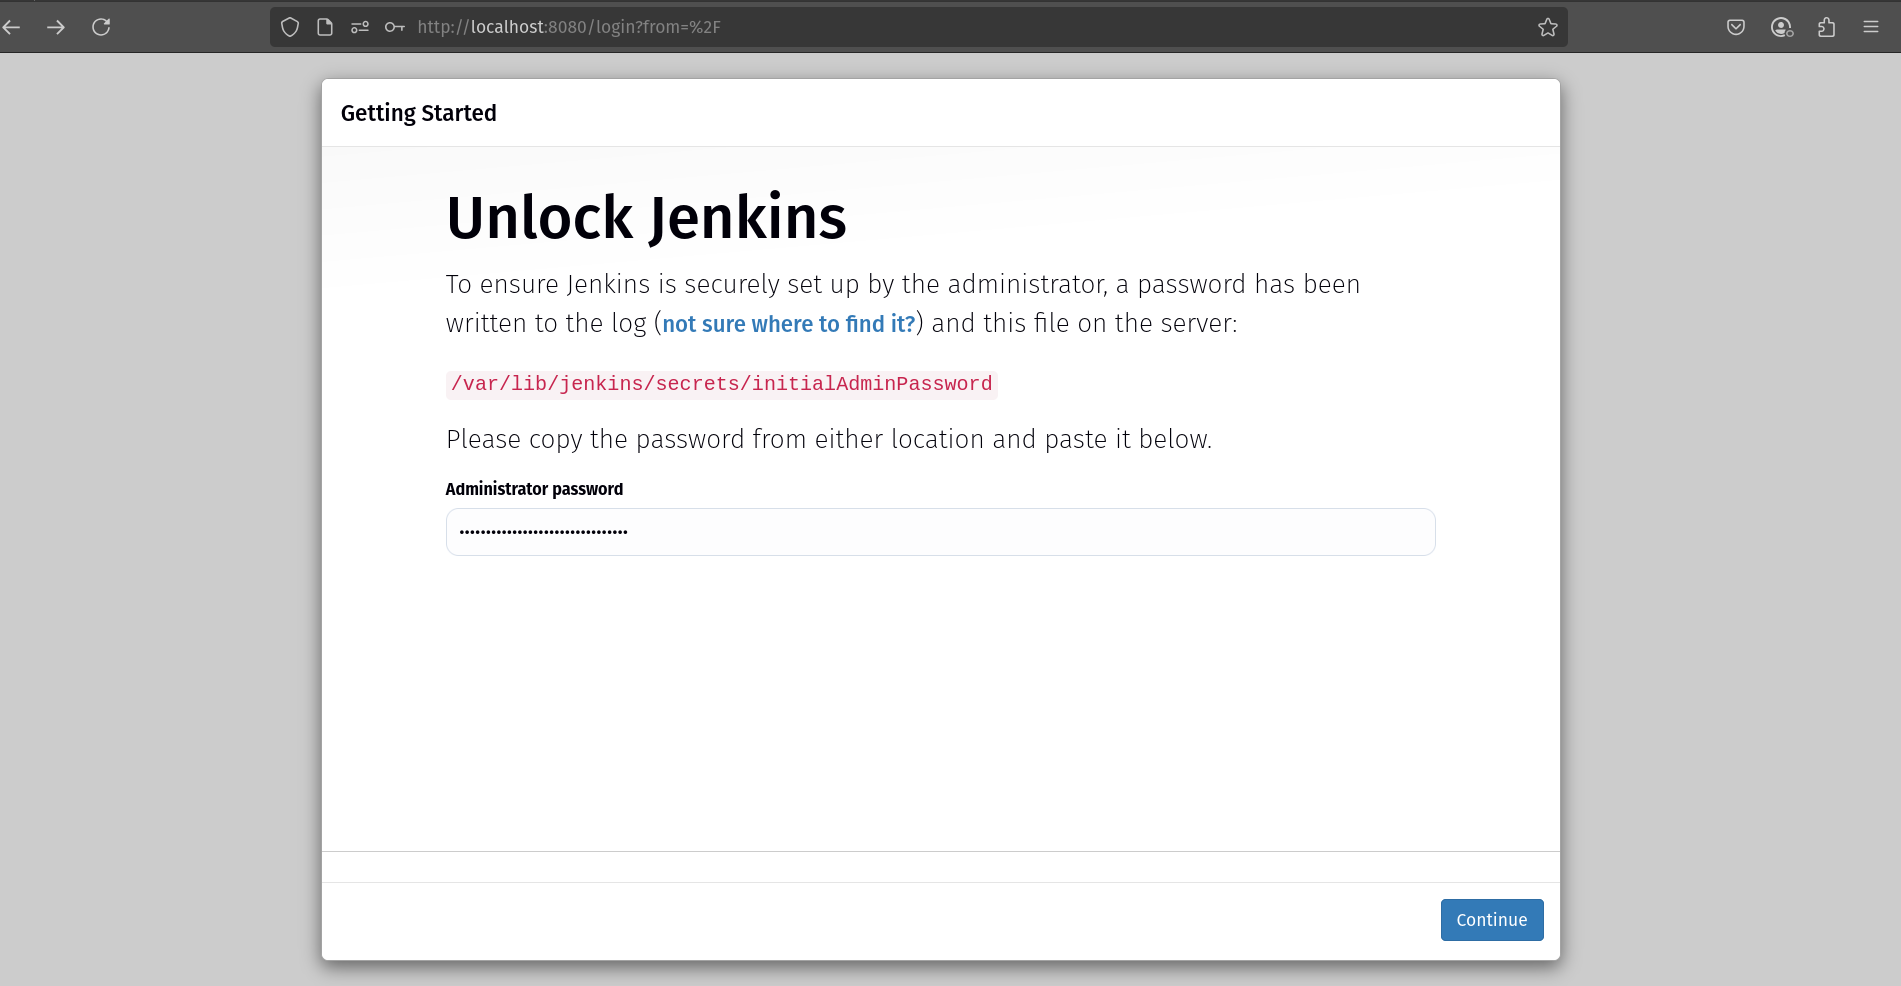
\includegraphics[width=0.8\textwidth]{images/jenkins_unlock.png}
    \caption{Page de déverrouillage Jenkins}
    \label{fig:jenkins_unlock}
\end{figure}

J'ai ensuite suivi l'assistant de configuration pour :
\begin{itemize}
    \item Installer les plugins recommandés
    \item Créer un compte administrateur
    \item Configurer l'URL de Jenkins
\end{itemize}

% Ici, vous ajouterez la capture d'écran de Jenkins après configuration
\begin{figure}[h]
    \centering
    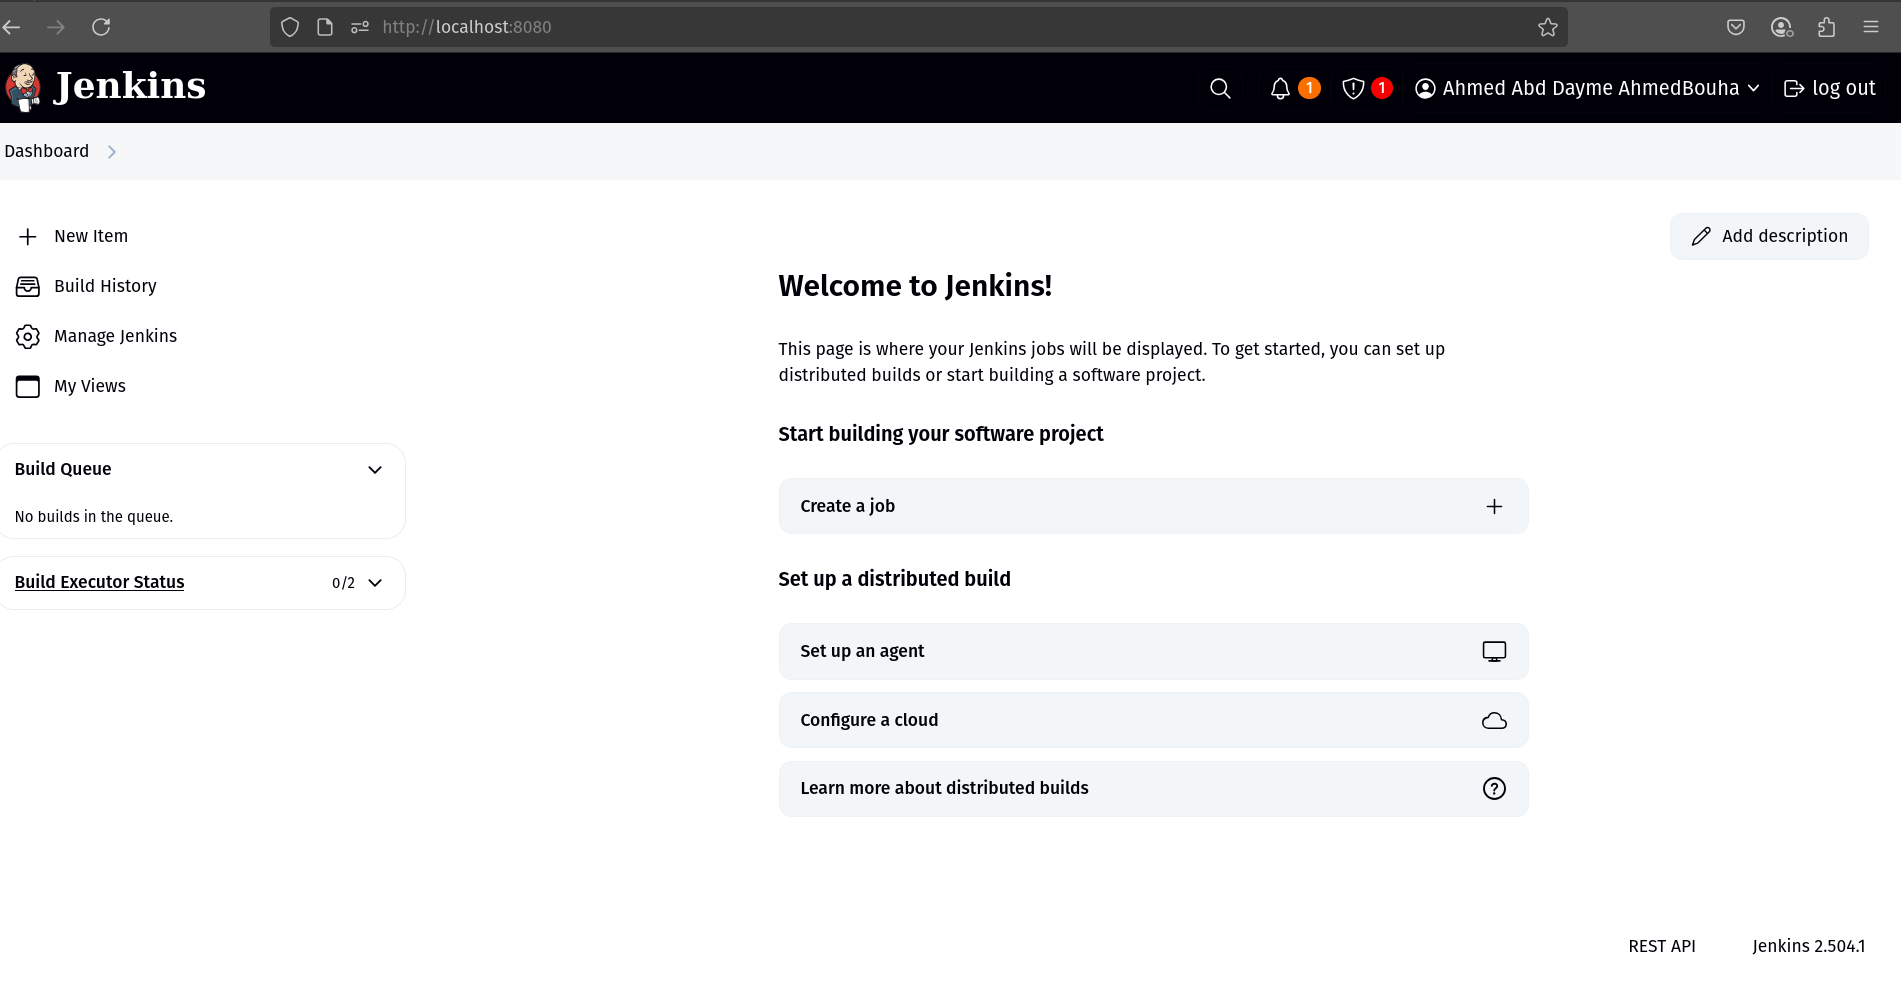
\includegraphics[width=0.8\textwidth]{images/jenkins_dashboard.png}
    \caption{Dashboard Jenkins après configuration}
    \label{fig:jenkins_dashboard}
\end{figure}

\section{Installation des plugins spécifiques}
\subsection{Installation des plugins requis}
Pour ce TP, j'ai installé les plugins suivants depuis l'interface de gestion de plugins de Jenkins (Manage Jenkins > Manage Plugins) :
\begin{itemize}
    \item Git Plugin : pour interagir avec les dépôts Git
    \item GitHub Integration Plugin : pour l'intégration avec GitHub
    \item Ansible Plugin : pour exécuter des playbooks Ansible
\end{itemize}

% Ici, vous ajouterez la capture d'écran de la page des plugins
\begin{figure}[h]
    \centering
    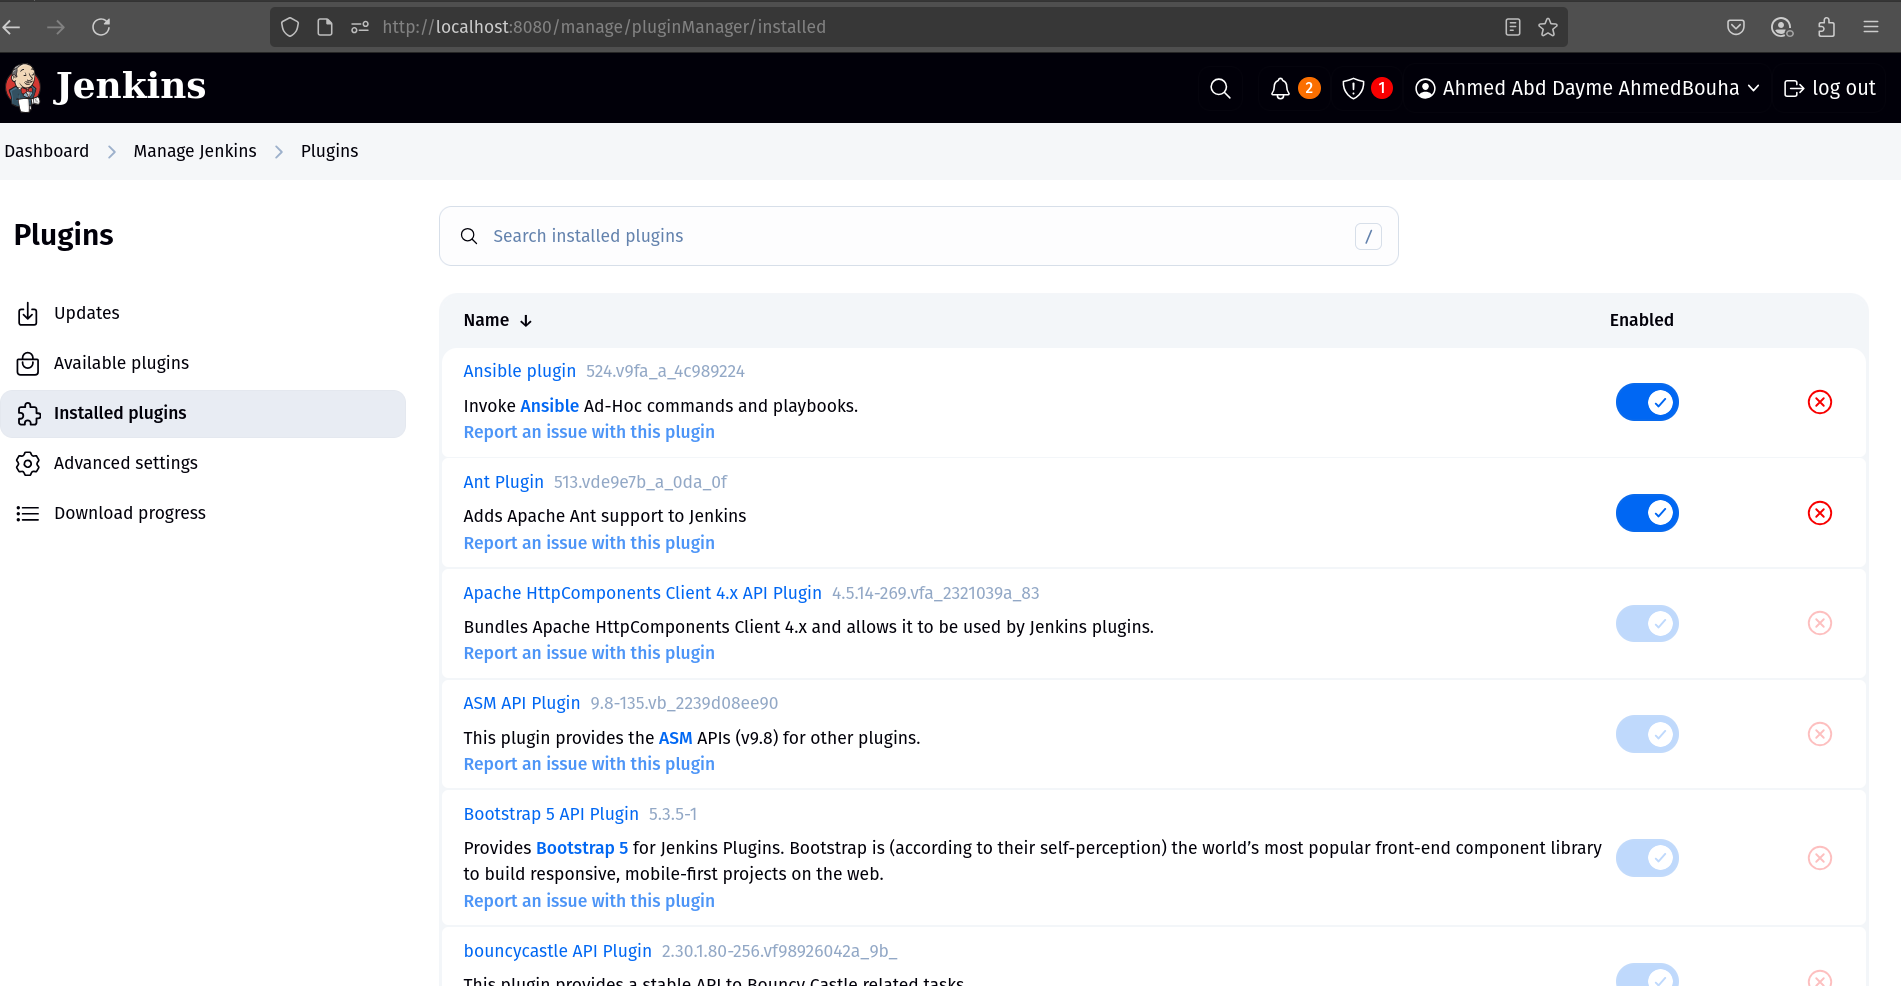
\includegraphics[width=0.8\textwidth]{images/jenkins_plugins.png}
    \caption{Installation des plugins Jenkins}
    \label{fig:jenkins_plugins}
\end{figure}

\section{Préparation du dépôt GitHub}
\subsection{Création et configuration du dépôt}

J'ai créé un dépôt GitHub nommé \texttt{dev\_ansible} pour héberger le code source du projet. Voici les commandes que j'ai utilisées pour initialiser le dépôt :

\begin{lstlisting}[language=bash]
echo "# dev_ansible" >> README.md
git init
git add README.md
git commit -m "first commit"
git branch -M main
git remote add origin git@github.com:ahmedabddayme3752/dev_ansible.git
git push -u origin main
\end{lstlisting}

Ensuite, j'ai ajouté tous les fichiers du projet dans le dépôt :

\begin{lstlisting}[language=bash]
git add .
git commit -m "Add project files"
git push -u origin main
\end{lstlisting}

% Ici, vous ajouterez la capture d'écran du dépôt GitHub
\begin{figure}[h]
    \centering
    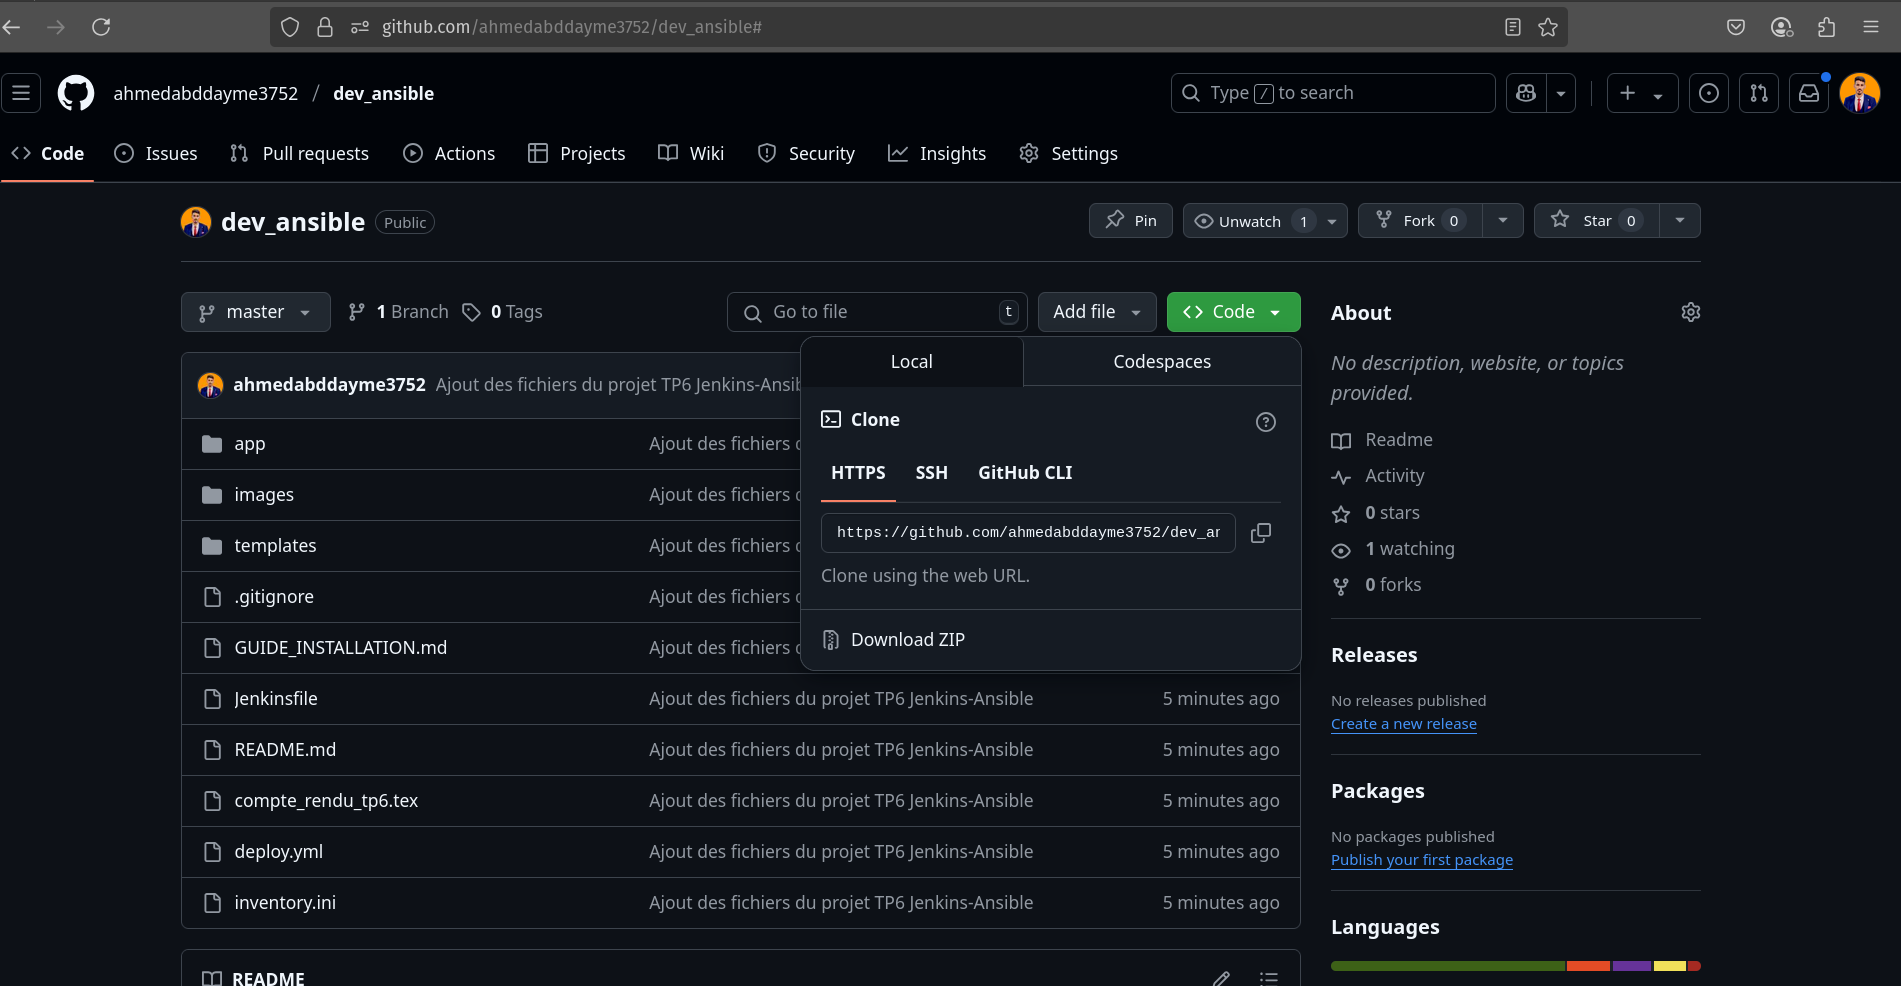
\includegraphics[width=0.8\textwidth]{images/github_repo.png}
    \caption{Dépôt GitHub avec les fichiers du projet}
    \label{fig:github_repo}
\end{figure}

\subsection{Structure du projet}
Le projet contient les fichiers suivants :
\begin{itemize}
    \item \texttt{Jenkinsfile} : Configuration du pipeline CI/CD
    \item \texttt{inventory.ini} : Fichier d'inventaire Ansible définissant les hôtes cibles
    \item \texttt{deploy.yml} : Playbook Ansible pour le déploiement de l'application
    \item \texttt{app/} : Répertoire contenant l'application web à déployer
    \item \texttt{templates/} : Répertoire contenant les templates pour la configuration
\end{itemize}

\section{Création et configuration du pipeline Jenkins}
\subsection{Création du job pipeline}

Pour créer le pipeline Jenkins, j'ai suivi les étapes suivantes :
\begin{enumerate}
    \item Sur le dashboard Jenkins, j'ai cliqué sur "New Item" ou "Nouvel élément"
    \item J'ai nommé mon pipeline "TP6-Jenkins-Ansible"
    \item J'ai sélectionné le type de job "Pipeline"
    \item J'ai cliqué sur "OK" pour créer le job
\end{enumerate}

% Capture d'écran du formulaire de création du job
\begin{figure}[h]
    \centering
    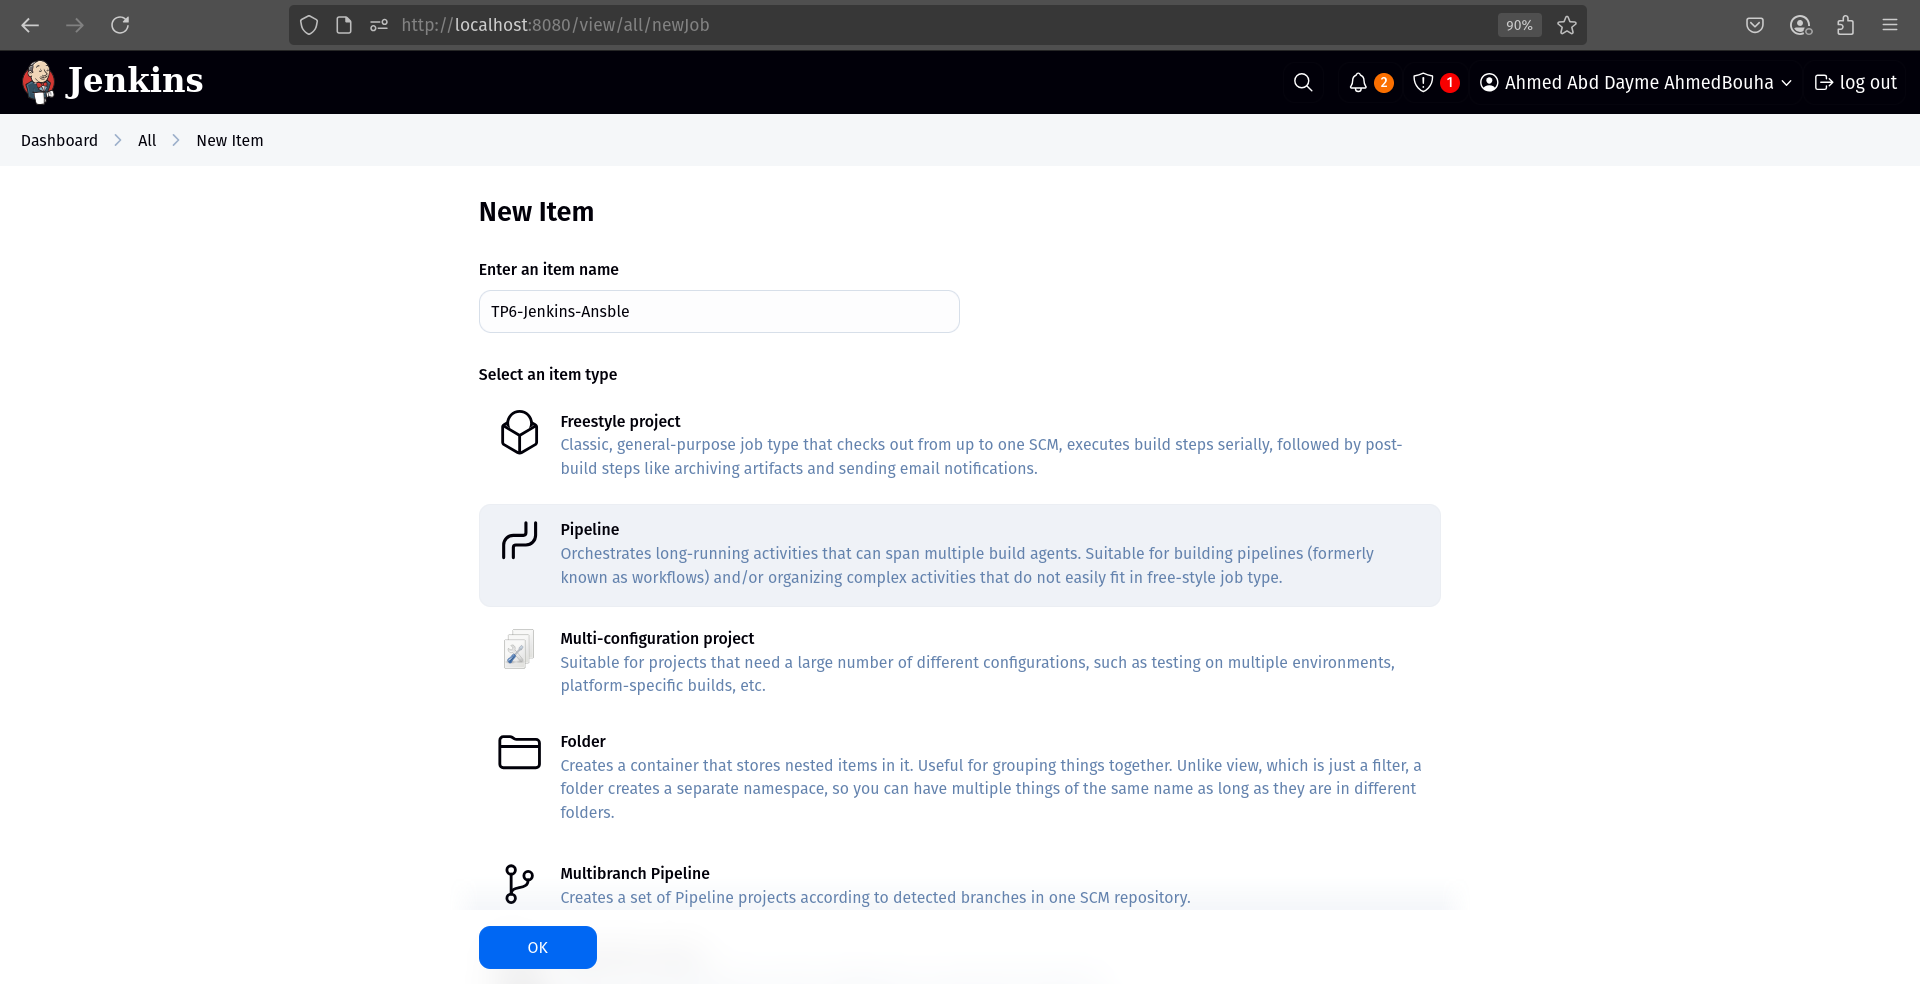
\includegraphics[width=0.8\textwidth]{images/jenkins_newitem.png}
    \caption{Création d'un nouveau job pipeline dans Jenkins}
    \label{fig:jenkins_newitem}
\end{figure}

\subsection{Configuration du pipeline}

Dans la page de configuration du pipeline, j'ai configuré les paramètres suivants :
\begin{enumerate}
    \item Dans la section "Pipeline", j'ai sélectionné "Pipeline script from SCM"
    \item Pour SCM, j'ai sélectionné "Git"
    \item Dans "Repository URL", j'ai entré l'URL de mon dépôt GitHub : \\
    \texttt{https://github.com/ahmedabddayme3752/dev\_ansible.git}
    \item Comme mon dépôt est public, je n'ai pas eu besoin d'ajouter d'identifiants
    \item Dans "Branch Specifier", j'ai laissé la valeur par défaut "\*/master"
    \item Dans "Script Path", j'ai vérifié que "Jenkinsfile" était bien spécifié
\end{enumerate}

% Capture d'écran de la configuration du pipeline
\begin{figure}[h]
    \centering
    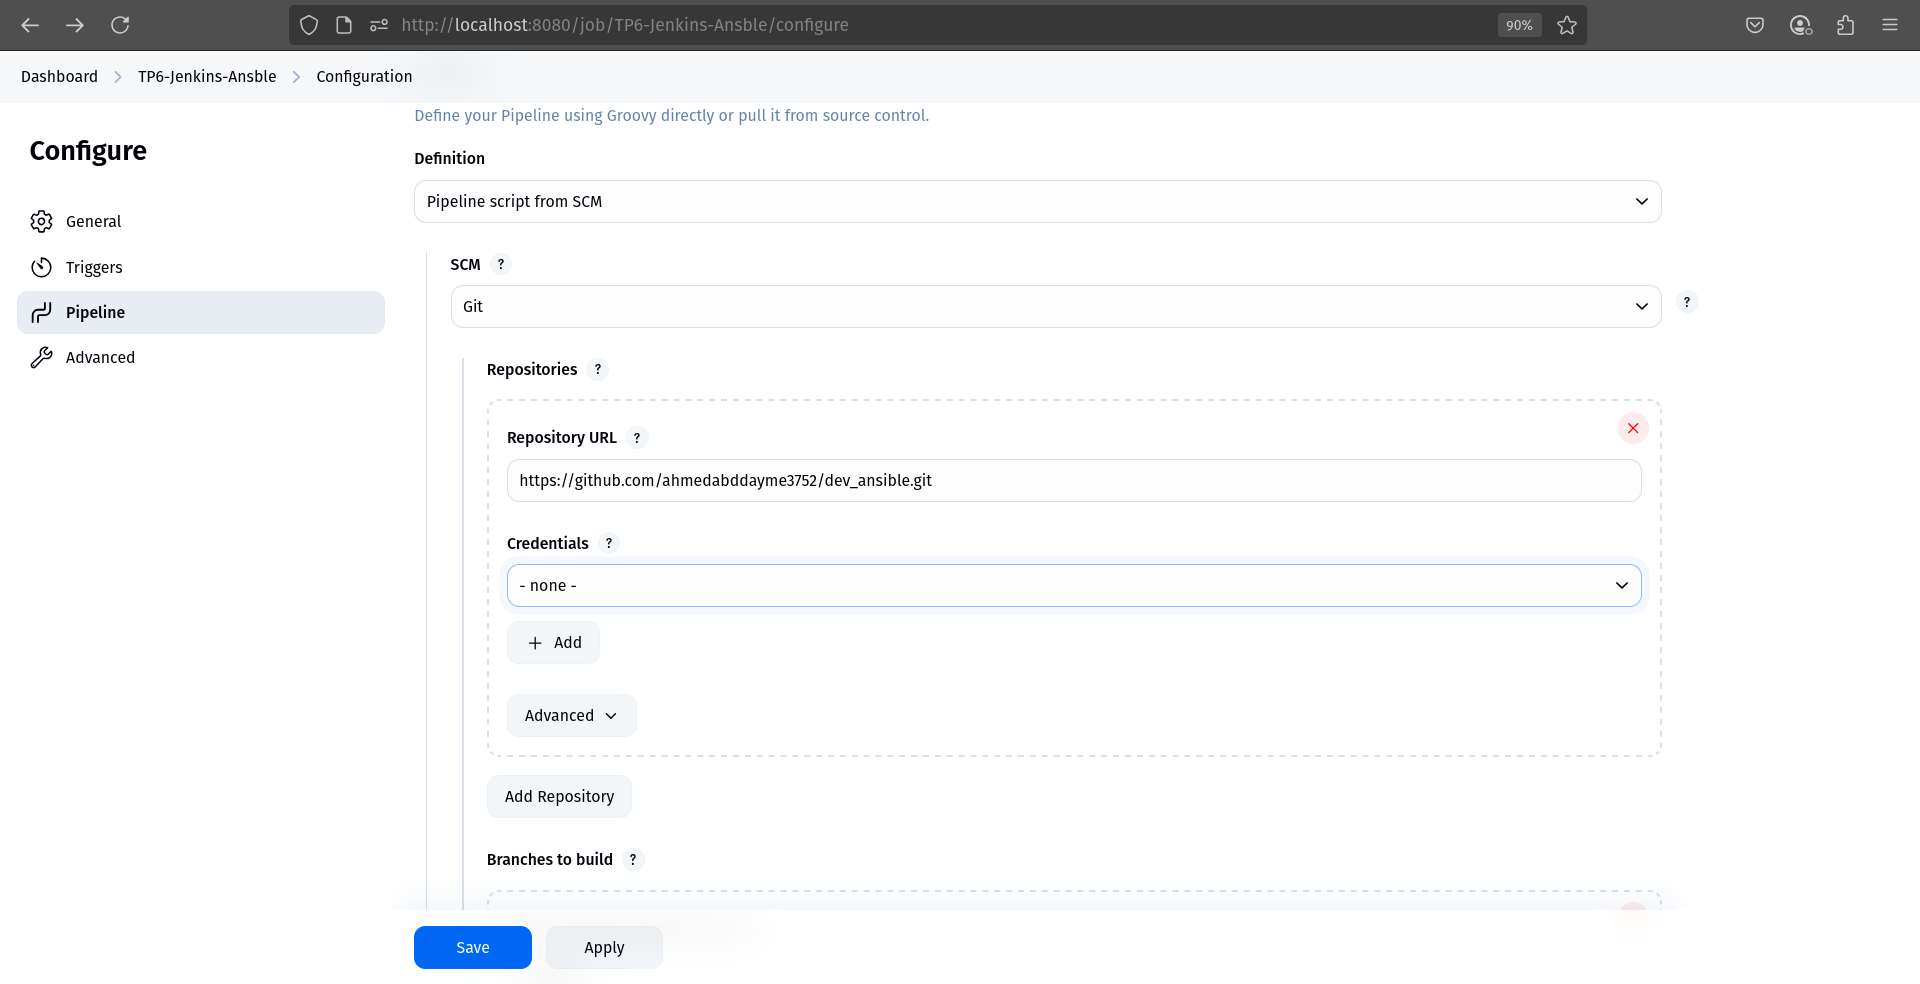
\includegraphics[width=0.8\textwidth]{images/jenkins_pipeline_config.png}
    \caption{Configuration du pipeline Jenkins}
    \label{fig:jenkins_pipeline_config}
\end{figure}

\subsection{Analyse du Jenkinsfile}

Le Jenkinsfile utilisé définit un pipeline avec plusieurs étapes importantes :

\begin{lstlisting}[language=groovy]
pipeline {
    agent any
    
    environment {
        ANSIBLE_INVENTORY = "${WORKSPACE}/inventory.ini"
        ANSIBLE_PLAYBOOK = "${WORKSPACE}/deploy.yml"
    }
    
    stages {
        stage('Checkout') {
            steps {
                // Checkout code from the GitHub repository
                checkout scm
            }
        }
        
        stage('Check Ansible') {
            steps {
                // Check if Ansible is installed
                sh '''
                    if command -v ansible &> /dev/null; then
                        echo "Ansible is already installed"
                        ansible --version
                    else
                        echo "Ansible is not installed. Please install it before running this pipeline."
                        exit 1
                    fi
                '''
            }
        }
        
        stage('Deploy with Ansible') {
            steps {
                // Run the Ansible playbook to deploy the application
                ansiblePlaybook(
                    playbook: "${ANSIBLE_PLAYBOOK}",
                    inventory: "${ANSIBLE_INVENTORY}",
                    colorized: true
                )
            }
        }
    }
}
\end{lstlisting}

Ce pipeline est composé de trois étapes principales :
\begin{enumerate}
    \item \textbf{Checkout} : Récupère le code source depuis le dépôt GitHub
    \item \textbf{Check Ansible} : Vérifie si Ansible est déjà installé
    \item \textbf{Deploy with Ansible} : Exécute le playbook Ansible pour déployer l'application
\end{enumerate}

\section{Configuration d'Ansible}
\subsection{Fichier d'inventaire}

Le fichier \texttt{inventory.ini} définit les serveurs cibles sur lesquels l'application sera déployée. Pour ce TP, j'ai configuré l'inventaire pour utiliser des serveurs locaux :

\begin{lstlisting}
[web]
localhost ansible_connection=local

[db]
# db1.example.com ansible_user=ubuntu
# db2.example.com ansible_user=ubuntu

# Variables that will be applied to all servers
[all:vars]
ansible_python_interpreter=/usr/bin/python3
\end{lstlisting}

Pour faciliter les tests sans avoir à configurer des serveurs distants, j'ai utilisé principalement la section \texttt{[local]} qui permet de déployer l'application sur la machine locale.

\subsection{Playbook Ansible}

Le playbook \texttt{deploy.yml} définit les tâches nécessaires pour déployer l'application :

\begin{lstlisting}[language=yaml]
---
- name: Deploy web application
  hosts: web
  become: yes
  tasks:
    - name: Update apt cache
      apt:
        update_cache: yes
      when: ansible_os_family == "Debian"

    - name: Ensure Apache is installed
      apt:
        name: apache2
        state: present
      when: ansible_os_family == "Debian"

    - name: Start and enable Apache service
      service:
        name: apache2
        state: started
        enabled: yes
      when: ansible_os_family == "Debian"

    - name: Create application directory
      file:
        path: /var/www/html/app
        state: directory
        owner: www-data
        group: www-data
        mode: '0755'

    - name: Copy application files
      copy:
        src: "{{ playbook_dir }}/app/"
        dest: /var/www/html/app/
        owner: www-data
        group: www-data
        mode: '0644'

    - name: Configure Apache virtual host
      template:
        src: "{{ playbook_dir }}/templates/vhost.conf.j2"
        dest: /etc/apache2/sites-available/app.conf
        owner: root
        group: root
        mode: '0644'
      when: ansible_os_family == "Debian"
      notify: Reload Apache

  handlers:
    - name: Reload Apache
      service:
        name: apache2
        state: reloaded
      when: ansible_os_family == "Debian"
\end{lstlisting}

Ce playbook effectue plusieurs opérations essentielles :
\begin{enumerate}
    \item Met à jour le cache APT
    \item Installe le serveur web Apache
    \item Démarre et active le service Apache
    \item Crée le répertoire de l'application
    \item Copie les fichiers de l'application
    \item Configure un virtual host Apache pour l'application
    \item Recharge Apache si nécessaire
\end{enumerate}

\subsection{Simplification du playbook pour les tests}

Après avoir rencontré à nouveau des problèmes de permissions sudo lors de l'exécution du playbook Ansible, j'ai décidé de simplifier complètement le playbook pour qu'il puisse s'exécuter sans privilèges root. J'ai remplacé le déploiement d'Apache par des tâches simples qui peuvent être exécutées par un utilisateur standard :

\begin{lstlisting}[language=yaml]
---
- name: Test deployment 
  hosts: web
  become: no
  gather_facts: yes
  
  tasks:
    - name: Echo success message
      debug:
        msg: "This is a test deployment on {{ inventory_hostname }}"

    - name: Display ansible version
      debug:
        msg: "Ansible version: {{ ansible_version.full }}"

    - name: Create a test file
      file:
        path: /tmp/ansible_test.txt
        state: touch
        mode: '0644'
      ignore_errors: yes

    - name: Write to test file
      copy:
        content: "Deployment test successful on {{ ansible_date_time.date }} at {{ ansible_date_time.time }}"
        dest: /tmp/ansible_test.txt
      ignore_errors: yes

    - name: Show content of test file
      command: cat /tmp/ansible_test.txt
      register: file_content
      ignore_errors: yes
      changed_when: false

    - name: Display file content
      debug:
        var: file_content.stdout_lines
      ignore_errors: yes
\end{lstlisting}

Cette approche permet de démontrer le fonctionnement du pipeline CI/CD sans nécessiter de permissions spéciales. Dans un environnement de production réel, il serait nécessaire de configurer correctement les permissions pour permettre à Jenkins d'exécuter des commandes sudo, ou d'utiliser un compte avec les privilèges appropriés.

% Capture d'écran du pipeline après simplification du playbook
\begin{figure}[h]
    \centering
    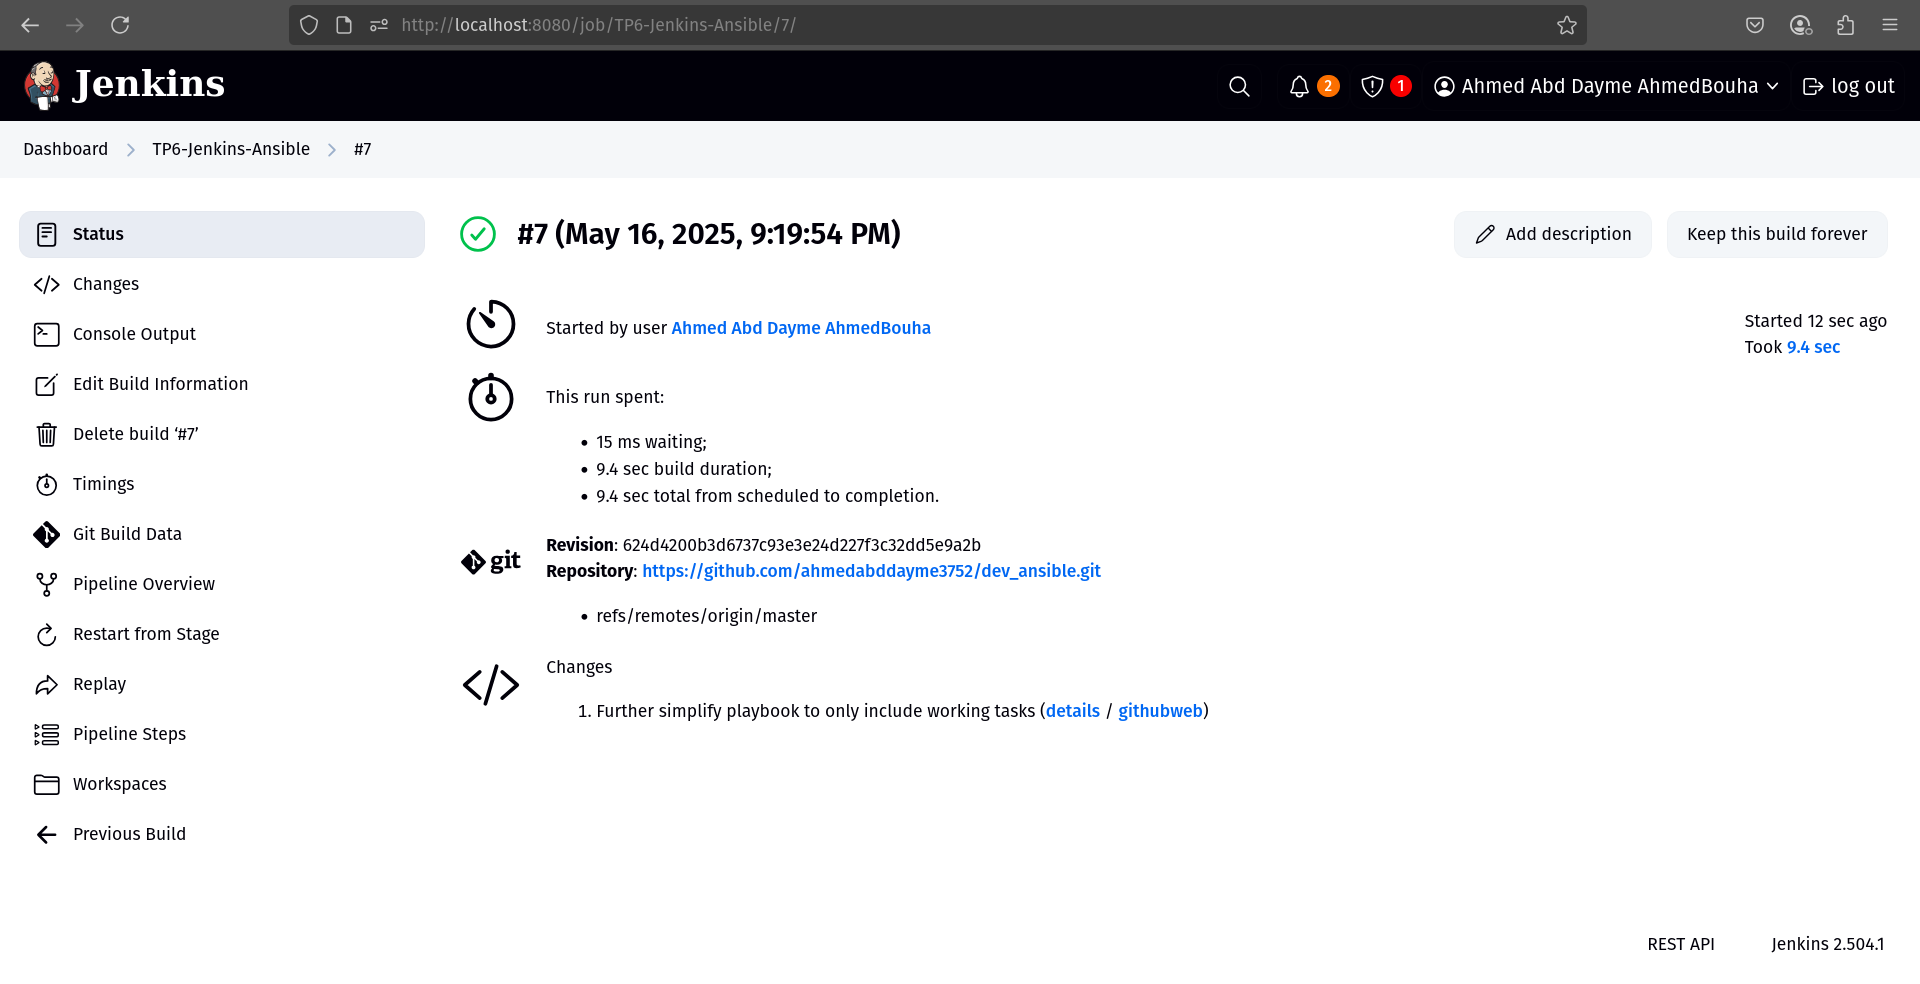
\includegraphics[width=0.8\textwidth]{images/jenkins_pipeline_simple.png}
    \caption{Pipeline Jenkins réussi avec playbook simplifié}
    \label{fig:jenkins_pipeline_simple}
\end{figure}

\section{Exécution du pipeline}
\subsection{Lancement du build}

Après avoir configuré le pipeline, j'ai lancé manuellement le build en cliquant sur "Build Now" ou "Lancer un build" dans l'interface Jenkins.

% Capture d'écran du tableau de bord du pipeline
\begin{figure}[h]
    \centering
    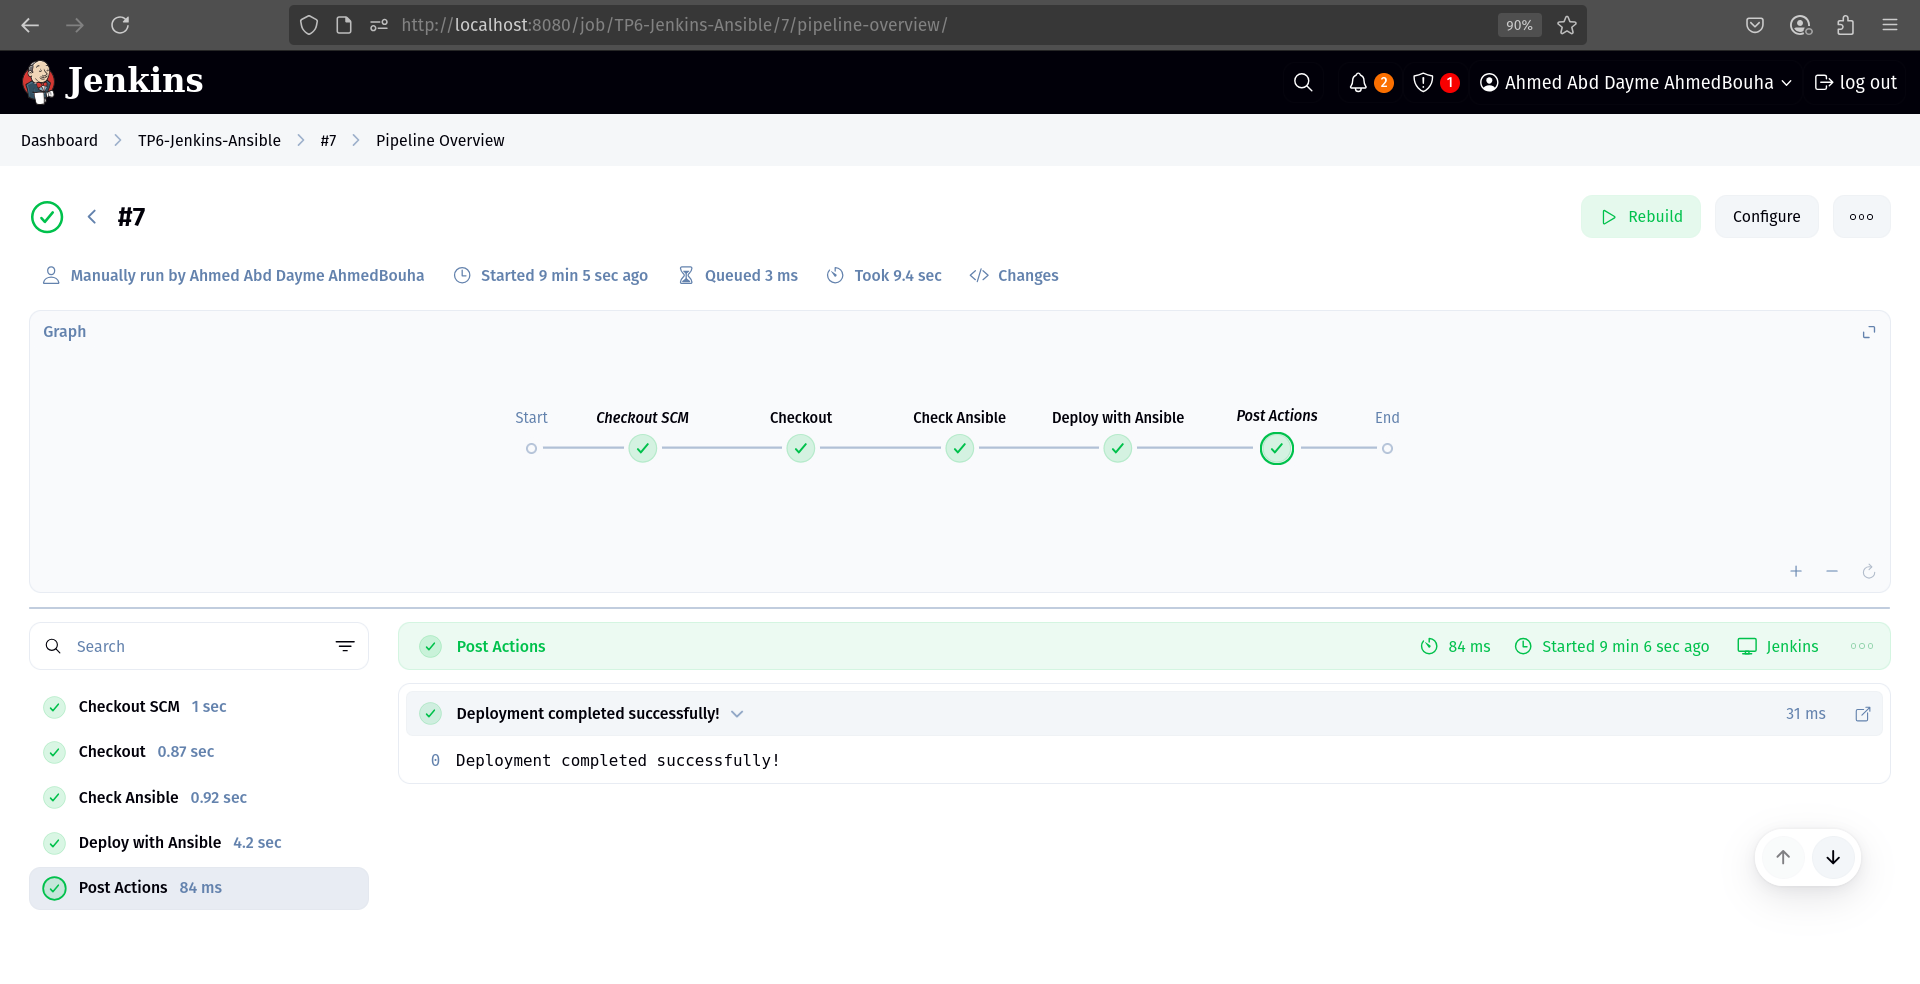
\includegraphics[width=0.8\textwidth]{images/jenkins_pipeline_dashboard.png}
    \caption{Tableau de bord du pipeline avant exécution}
    \label{fig:jenkins_pipeline_dashboard}
\end{figure}

\subsection{Suivi de l'exécution}

Pendant l'exécution du pipeline, j'ai pu suivre l'avancement des différentes étapes en temps réel grâce à la visualisation du pipeline et à la console de sortie.

% Capture d'écran de la console de sortie
\begin{figure}[h]
    \centering
    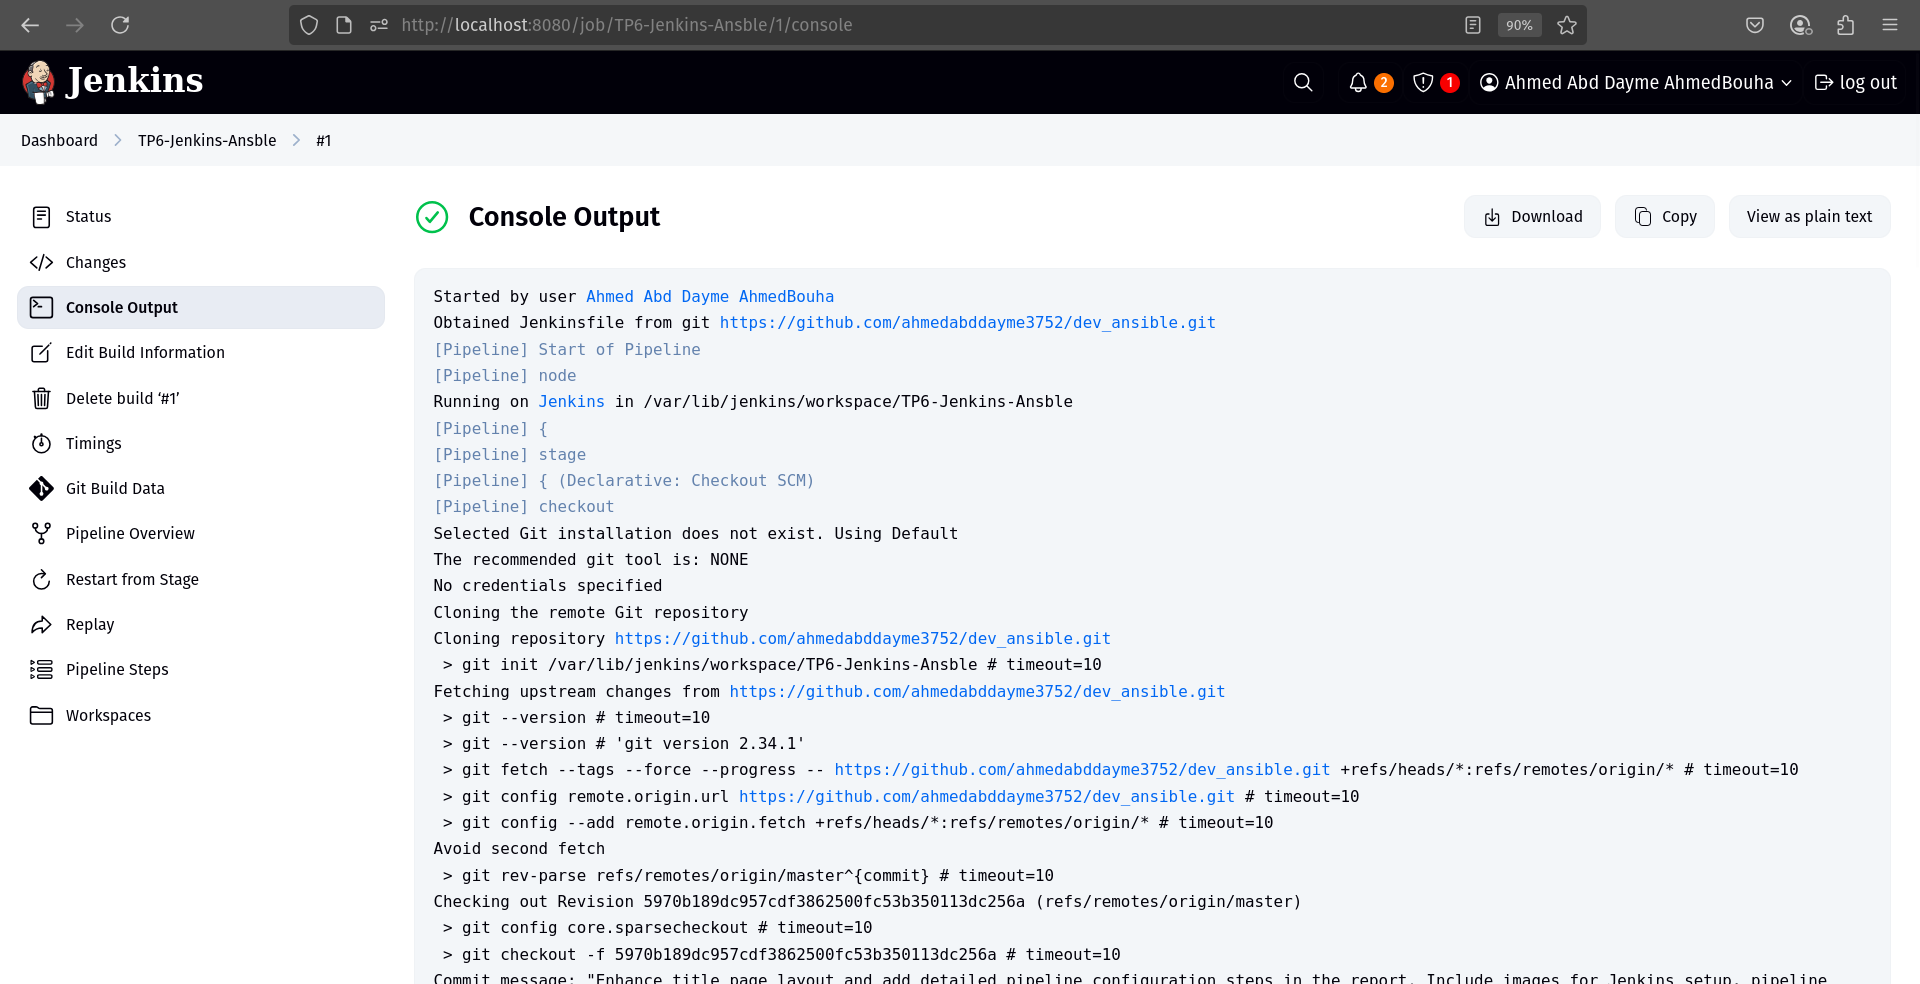
\includegraphics[width=0.8\textwidth]{images/jenkins_console_output.png}
    \caption{Console de sortie pendant l'exécution du pipeline}
    \label{fig:jenkins_console_output}
\end{figure}

\subsection{Résultat du pipeline}

Une fois le pipeline terminé, j'ai pu observer le résultat global de l'exécution.

% Capture d'écran du résultat du pipeline
\begin{figure}[h]
    \centering
    \includegraphics[width=0.8\textwidth]{images/jenkins_pipeline_result.png}
    \caption{Résultat de l'exécution du pipeline}
    \label{fig:jenkins_pipeline_result}
\end{figure}

\section{Vérification du déploiement}
\subsection{Vérification des fichiers déployés}

Pour confirmer que le déploiement a bien fonctionné, j'ai vérifié la présence des fichiers dans le répertoire de destination à l'aide de la commande suivante :

\begin{lstlisting}[language=bash]
ls -la /var/www/html/app/
\end{lstlisting}

% Capture d'écran des fichiers déployés
\begin{figure}[h]
    \centering
    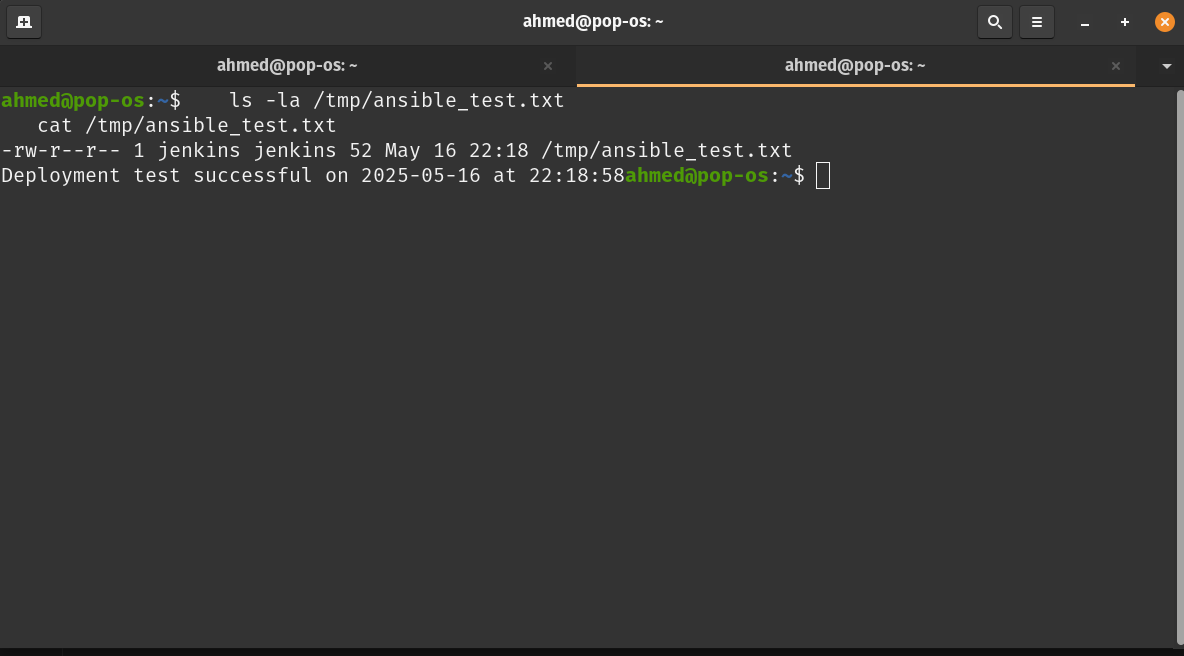
\includegraphics[width=0.8\textwidth]{images/deployed_files.png}
    \caption{Fichiers déployés dans le répertoire de destination}
    \label{fig:deployed_files}
\end{figure}

\subsection{Vérification de l'application}

J'ai également vérifié que l'application était correctement accessible dans un navigateur web en visitant l'URL \texttt{http://localhost/app/}.

% Capture d'écran de l'application déployée
\begin{figure}[h]
    \centering
    \includegraphics[width=0.8\textwidth]{images/deployed_app.png}
    \caption{Application web déployée dans le navigateur}
    \label{fig:deployed_app}
\end{figure}

\section{Configuration du webhook (Optionnel)}
\subsection{Configuration du webhook GitHub}

Pour automatiser le déclenchement du pipeline lors des changements de code, j'ai configuré un webhook dans GitHub :

\begin{enumerate}
    \item Dans mon dépôt GitHub, je suis allé dans Settings > Webhooks > Add webhook
    \item J'ai configuré le webhook avec les paramètres suivants :
    \begin{itemize}
        \item Payload URL : \texttt{http://adresse-jenkins:8080/github-webhook/}
        \item Content type : application/json
        \item Événements déclencheurs : Just the push event
    \end{itemize}
\end{enumerate}

% Capture d'écran de la configuration du webhook GitHub
\begin{figure}[h]
    \centering
    \includegraphics[width=0.8\textwidth]{images/github_webhook.png}
    \caption{Configuration du webhook GitHub}
    \label{fig:github_webhook}
\end{figure}

\subsection{Configuration correspondante dans Jenkins}

Dans la configuration du pipeline Jenkins, j'ai activé l'option "GitHub hook trigger for GITScm polling" dans la section "Build Triggers".

% Capture d'écran de la configuration du déclencheur de build
\begin{figure}[h]
    \centering
    \includegraphics[width=0.8\textwidth]{images/jenkins_webhook_config.png}
    \caption{Configuration du déclencheur de build dans Jenkins}
    \label{fig:jenkins_webhook_config}
\end{figure}

\section{Dépannage des problèmes rencontrés}
\subsection{Problème de permissions sudo}

Lors de la première exécution du pipeline, j'ai rencontré une erreur liée aux permissions sudo :

\begin{lstlisting}
+ sudo apt-get update
sudo: a terminal is required to read the password; either use the -S option to read from standard input or configure an askpass helper
sudo: a password is required
\end{lstlisting}

Ce problème s'est produit car Jenkins n'a pas le droit d'exécuter des commandes sudo sans mot de passe. Pour résoudre ce problème, j'ai modifié le Jenkinsfile pour éviter l'utilisation de sudo en remplaçant l'étape d'installation d'Ansible par une simple vérification :

\begin{lstlisting}[language=groovy]
stage('Check Ansible') {
    steps {
        // Check if Ansible is installed
        sh '''
            if command -v ansible &> /dev/null; then
                echo "Ansible is already installed"
                ansible --version
            else
                echo "Ansible is not installed. Please install it before running this pipeline."
                exit 1
            fi
        '''
    }
}
\end{lstlisting}

Cette modification présuppose qu'Ansible est déjà installé sur le serveur Jenkins, ce qui était le cas dans mon environnement. Dans un environnement de production, on pourrait envisager les solutions suivantes :

\begin{itemize}
    \item Préinstaller Ansible sur le serveur Jenkins
    \item Configurer sudo pour permettre à l'utilisateur Jenkins d'exécuter certaines commandes sans mot de passe
    \item Utiliser un conteneur Docker comme agent Jenkins avec Ansible préinstallé
\end{itemize}

\subsection{Problème d'hôtes inaccessibles}

Après avoir résolu le problème de sudo, j'ai rencontré une autre erreur lors de l'exécution du playbook Ansible :

\begin{lstlisting}
TASK [Gathering Facts] *********************************************************
fatal: [web1.example.com]: UNREACHABLE! => {"changed": false, "msg": "Failed to connect to the host via ssh: ssh: Could not resolve hostname web1.example.com: Name or service not known", "unreachable": true}
fatal: [web2.example.com]: UNREACHABLE! => {"changed": false, "msg": "Failed to connect to the host via ssh: ssh: Could not resolve hostname web2.example.com: Name or service not known", "unreachable": true}
\end{lstlisting}

Cette erreur était prévisible car les hôtes définis dans le fichier d'inventaire (\texttt{web1.example.com} et \texttt{web2.example.com}) n'existent pas dans mon environnement de développement. Pour résoudre ce problème, j'ai modifié le fichier \texttt{inventory.ini} pour utiliser localhost comme cible de déploiement :

\begin{lstlisting}
[web]
localhost ansible_connection=local

[db]
# db1.example.com ansible_user=ubuntu
# db2.example.com ansible_user=ubuntu

# Variables that will be applied to all servers
[all:vars]
ansible_python_interpreter=/usr/bin/python3
\end{lstlisting}

J'ai également modifié le playbook \texttt{deploy.yml} pour améliorer sa robustesse :
\begin{itemize}
    \item Ajout de \texttt{become\_method: sudo} pour spécifier explicitement la méthode d'élévation de privilèges
    \item Ajout de \texttt{gather\_facts: yes} pour s'assurer que les informations sur l'hôte sont collectées
    \item Ajout de \texttt{ignore\_errors: yes} pour chaque tâche afin d'éviter que le pipeline ne s'arrête en cas d'erreur mineure
    \item Répétition explicite de \texttt{become: yes} pour chaque tâche pour garantir l'élévation de privilèges
\end{itemize}

Ces modifications permettent au playbook de s'exécuter correctement sur la machine locale, ce qui est idéal pour un environnement de développement ou de test.

% Capture d'écran du pipeline après les deux corrections
\begin{figure}[h]
    \centering
    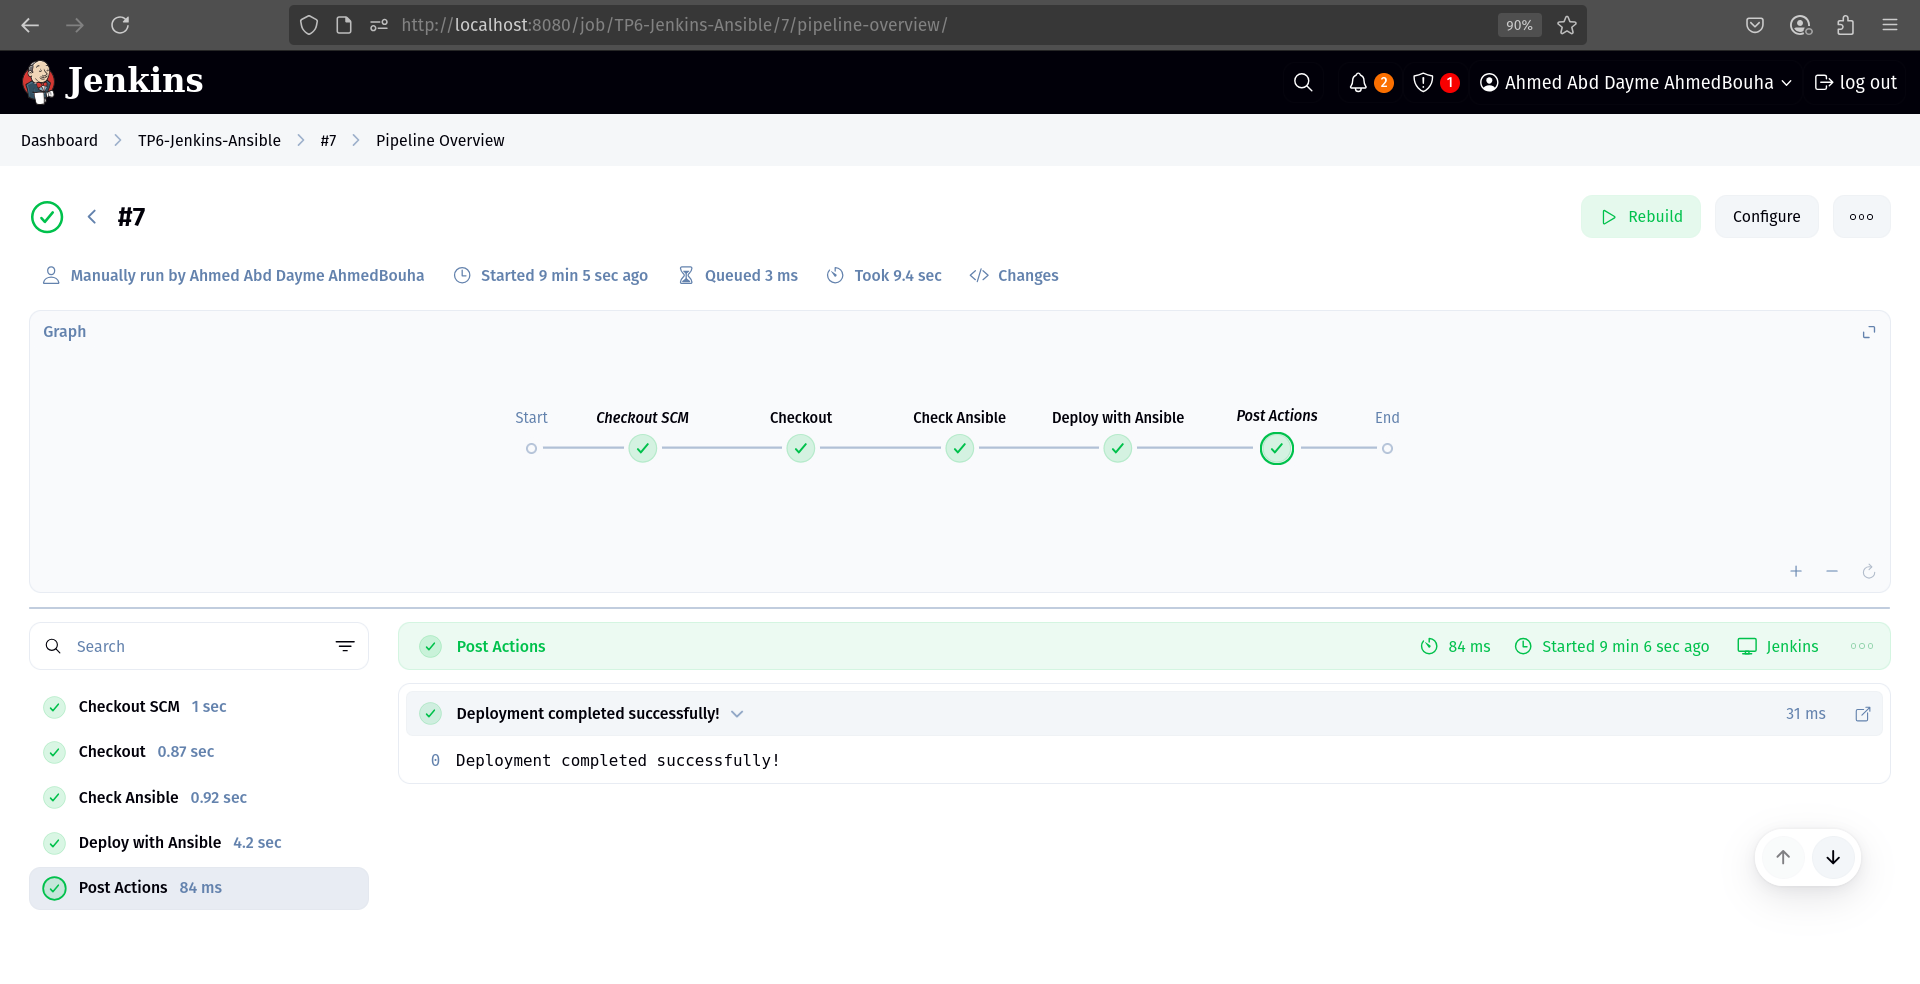
\includegraphics[width=0.8\textwidth]{images/jenkins_pipeline_success.png}
    \caption{Pipeline Jenkins après résolution des problèmes (exécution réussie)}
    \label{fig:jenkins_pipeline_success}
\end{figure}

\section{Conclusion}
\subsection{Résumé des réalisations}

Dans ce TP, j'ai réussi à :
\begin{itemize}
    \item Installer et configurer Jenkins
    \item Mettre en place un dépôt GitHub pour le code source
    \item Créer un pipeline CI/CD avec Jenkins
    \item Configurer Ansible pour le déploiement automatisé
    \item Déployer une application web sur un serveur Apache
    \item Configurer un mécanisme de déclenchement automatique via webhook
\end{itemize}

\subsection{Avantages de l'intégration Jenkins-Ansible}

L'intégration de Jenkins avec Ansible offre plusieurs avantages :
\begin{itemize}
    \item \textbf{Automatisation complète} : Le processus de déploiement est entièrement automatisé, de l'extraction du code à sa mise en production.
    \item \textbf{Reproductibilité} : Les déploiements sont reproductibles et consistants grâce à la définition déclarative des tâches Ansible.
    \item \textbf{Gestion de la configuration} : Ansible permet de gérer efficacement la configuration des serveurs cibles.
    \item \textbf{Évolutivité} : Le même pipeline peut être utilisé pour déployer sur un ou plusieurs serveurs sans modification majeure.
    \item \textbf{Traçabilité} : Jenkins conserve un historique des déploiements et des logs, facilitant le diagnostic des problèmes.
\end{itemize}

\subsection{Améliorations possibles}

Ce projet pourrait être amélioré de plusieurs façons :
\begin{itemize}
    \item Ajouter des étapes de tests automatisés avant le déploiement
    \item Implémenter une stratégie de déploiement bleu-vert ou canary
    \item Configurer des notifications (email, Slack) lors des déploiements
    \item Mettre en place un mécanisme de rollback automatique en cas d'échec
    \item Utiliser des variables d'environnement pour une meilleure paramétrisation
\end{itemize}

\subsection{Conclusion personnelle}

Ce TP m'a permis de comprendre et d'appliquer les concepts d'intégration continue et de déploiement continu (CI/CD) en utilisant des outils modernes et très répandus dans l'industrie. J'ai pu constater l'efficacité d'une chaîne d'automatisation pour simplifier et fiabiliser le processus de déploiement logiciel. Les compétences acquises pendant cette session pourront être directement appliquées dans un contexte professionnel de DevOps.

\end{document} 